\begin{center}
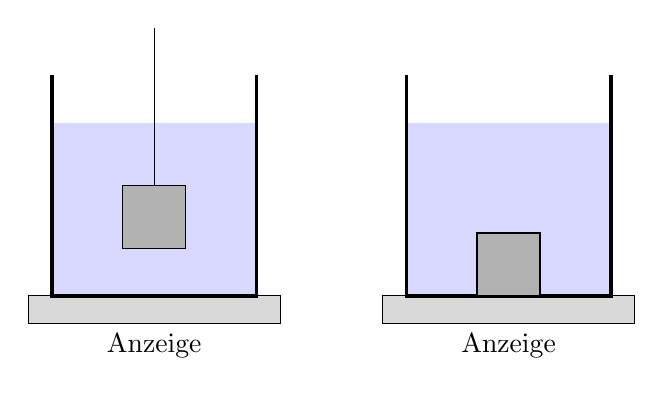
\begin{tikzpicture}[>=stealth]
 \draw[fill=gray!30] (-0.3,-0.35) rectangle (2.9,0);
 \node[below] at (1.3,-0.35) {Anzeige \mEiO};
 \fill[blue!15] (0,0) rectangle (2.6,2.2);
 \draw[very thick] (0,2.8) -- (0,0) -- (2.6,0) -- (2.6,2.8);
 \draw (1.3,3.4) -- (1.3,1.4);
 \draw[fill=gray!60] (0.9,0.6) rectangle (1.7,1.4);
 \draw[fill=gray!30] (4.2,-0.35) rectangle (7.4,0);
 \node[below] at (5.8,-0.35) {Anzeige \mBoO};
 \fill[blue!15] (4.5,0) rectangle (7.1,2.2);
 \draw[very thick] (4.5,2.8) -- (4.5,0) -- (7.1,0) -- (7.1,2.8);
 \draw[fill=gray!60] (5.4,0) rectangle (6.2,0.8);
\end{tikzpicture}
\end{center}

Hält man den Würfel ins Wasser, drückt das Wasser mit der Auftriebskraft $F_\text{A}$ auf den Würfel nach oben. Nach dem Wechselwirkungsprinzip drückt der Würfel mit gleich grosser Kraft auf das Wasser und damit auf die Waage. Die Anzeige $m_1 = \mEiO$ ist also die Masse des verdrängten Wassers, $F_\text{A} = m_1\,g = \rho_\text{W}\,V\,g$. Das Volumen des Würfels ist damit
\begin{align}
 V &= \VWF = \frac{\mEi}{\rhoW} = \VW
\end{align}
mit $\rho_\text{W} = \rhoWO$ (FoTaBe S.~187). Steht der Würfel auf dem Boden, trägt die Waage sein ganzes Gewicht; die Anzeige $m_2 = \mBoO$ ist seine Masse. Seine Dichte ist
\begin{align}
 \rho &= \frac{m_2}{V} = \rhoMF \\
   &= \frac{\mBo}{\mEi}\cdot\rhoW \\
   &= \rhoM \approx \result{\rhoMP{0}{2}}
\end{align}
Nach FoTaBe S.~187 besteht der Würfel aus \result{\text{Kupfer}} ($\rho = \rhoCuO$); Nickel ($\rho = \rhoNiO$) wäre mit diesen Messwerten nicht zu unterscheiden.
